
\ifintegriereaufgaben
\section*{Funktionenr�ume und Bestapproximation Aufgaben}\label{MA2-funktionenraeume-und-bestapproximation-aufgaben}

Erkl�rungen und Beispiele, die zur Bearbeitung der Aufgaben hilfreich sind, finden Sie im Skript\wennreferenzvorhanden{MA2-funktionenraeume-und-bestapproximation}{ (Abschnitt \abschnittsverweis{MA2-funktionenraeume-und-bestapproximation})} und, falls Sie nicht weiterkommen, schauen Sie \hyperref[MA2-funktionenraeume-und-bestapproximation-loesungen]{hier}.
\else
\section{Funktionenr�ume und Bestapproximation Aufgaben}\label{MA2-funktionenraeume-und-bestapproximation-aufgaben}

Regeln und Beispiele zu diesen Aufgaben finden Sie im Skript. Die L�sungen finden Sie \hyperref[MA2-funktionenraeume-und-bestapproximation-loesungen]{hier}.
\fi

\begin{exercisebox}[Gram-Schmidtsches Orthogonalisierungsverfahren]
	Gegeben sind drei linear unabh�ngige Vektoren. Bestimmen Sie ein Orthonormalsystem.
	\[
		\boldsymbol v_1 = \left( \begin{array}{c} 1 \\ i \\ 0 \\ 0 \end{array}\right)\,,
		\boldsymbol v_2 = \left( \begin{array}{c} i \\ 0 \\ 0 \\ i \end{array}\right)\,,
		\boldsymbol v_3 = \left( \begin{array}{c} 1 \\ 0 \\ 1 \\ 0 \end{array}\right)\,.
	\]
%	\begin{itemize}
%		\item[(a)] Bestimmen Sie zu $\boldsymbol v_1$ einen Vektor $\boldsymbol e_1$ mit
%			\[
%			\boldsymbol e_1 \parallel \boldsymbol v_1 \land \|\boldsymbol e_1\| = 1\,.\]
%		\item[(b)] Bestimmen Sie zu $\boldsymbol v_2$ einen Vektor $\boldsymbol e_2$ mit
%			\[
%			\boldsymbol e_2 \perp \boldsymbol e_1  \land \|\boldsymbol e_2\| = 1\,.\]
%		\item[(c)] Bestimmen Sie zu $\boldsymbol v_3$ einen Vektor $\boldsymbol e_3$ mit
%			\[
%			\boldsymbol e_3 \perp \boldsymbol e_i, \; i=1,2   \land \|\boldsymbol e_3\| = 1\,.\]
%		\item[(d)] Erg�nzen Sie die Vektoren $ \boldsymbol e_1, \boldsymbol e_2$ und $\boldsymbol e_3$ zu einer Basis von $\mathbb C^4$.
%	\end{itemize}

%\vspace{0.3cm}
%{\bf L�sung:} \newline
\end{exercisebox}
\begin{exercisebox}[Basis] %https://www.lntwww.de/Aufgaben:Aufgabe_4.1:_Zum_Gram-Schmidt-Verfahren
	Bei der Digitalsignal�bertragung werden energiebegrenzte Signale betrachtet. Das Skalarprodukt zweier Signale bzw. die Norm eines Signals sind hierbei wie folgt definiert:
	\begin{eqnarray*}
		\langle s_i, s_k\rangle &=& \int\limits_{-\infty}^{\infty} s_i(t) \cdot s_k(t) \, \mathrm{d}t\,,\\[1ex]
		\|s\| &=& \sqrt{\langle s,s \rangle}\,.
	\end{eqnarray*}
	Betrachten Sie die folgenden drei energiebegrenzten Signale:
	\begin{center}
	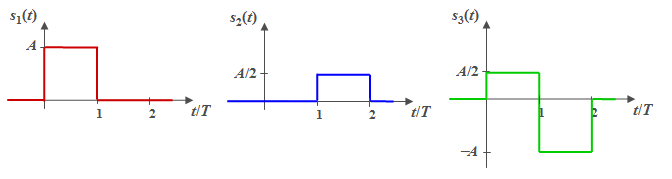
\includegraphics[width=0.7\textwidth]{../Mathematik_2/Bilder/funktionenraum_rechtecksignale_linearkombination.png}
\end{center}
	\begin{itemize}
		\item[(a)] Wie lauten die Abbildungsvorschriften der Signale $s_1, s_2$ und $s_3$?
		\item[(b)] Berechnen Sie die Normen der Signale $s_1$ und $s_2$.
		\item[(c)] Konstruieren Sie aus den Signalen $s_1$ und $s_2$ ein Orthonormalsystem.
		\item[(d)] Zerlegen Sie das Signal $s_3$ bez�glich des Orthonormalsystems und bestimmen Sie die vektoriellen Repr�sentanten der Ausgangssignale bez�glich des Orthonormalsystems.
	\end{itemize}
\end{exercisebox}


\begin{exercisebox}[Bestapproximation] %A.Z. Anwendungen
	Gegeben seien die Funktionen $f_1, f_2, f_3 \in \mathcal C([-\pi,\pi], \mathbb R)$ mit
	\[ f_1: x\mapsto 1, \quad f_2: x\mapsto \cos(x), \quad f_3: x\mapsto \sin(x)\]
	\begin{itemize}
		\item[(a)] Zeigen Sie, dass die Funktionen paarweise orthogonal sind bez�glich des Skalarprodukts
			\[ \langle f, g\rangle : = \int_{-\pi}^{\pi} f(x) \cdot g(x) \, \mathrm{d}x \]
		\item[(b)] Berechnen Sie die Bestapproximation $\tilde f \in \mathcal C([-\pi,\pi],\mathbb R)$ von $f:x\mapsto x^2$ bez�glich $f_i$, $i=1,2,3$ und zeichnen Sie $f$ und $\tilde f$.
		\item[(c)] Zeigen Sie, dass die folgenden Funktionen orthogonal sind\[ \cos(k\cdot x), \, k\in \mathbb N_0, \quad \sin(k\cdot x),  \, k\in \mathbb N\,.\]
	\end{itemize}

%\vspace{0.3cm}
%{\bf L�sung:} \newline
%\begin{itemize}
%	\item[(a)] $||f_1||=2\pi, \quad ||f_2||=\pi, \quad ||f_3|| = \pi $
%	\item[(b)] Es gilt \[ \langle f_1, f\rangle = \displaystyle{ \frac{2\pi^3}{3}}, \; \langle f_2, f\rangle = -4\pi,  \; \langle f_3, f\rangle = 0 \]
%		Also folgt \[ \tilde f(x) = \sum\limits_{k=1}^3 \frac{\langle f_k, f\rangle}{||f_k||^2} f_k = \frac{\pi^2}{3} - 4\cos(x)\,.\]
%	\item[(c)]  Man verwendet die Formeln
%		\begin{eqnarray*}
%			\cos(\alpha)\cdot \cos(\beta) &=& \frac12 \left( \cos( \alpha - \beta) + \cos(\alpha + \beta)\right) \\
%			\sin(\alpha)\cdot \sin(\beta) &=& \frac12 \left( \cos( \alpha - \beta) - \cos(\alpha + \beta)\right) \\
%			\sin(\alpha)\cdot \cos(\beta) &=& \frac12 \left( \sin( \alpha - \beta) + \sin(\alpha + \beta)\right)
%		\end{eqnarray*}
%	\end{itemize}
\end{exercisebox}

%\subsection{Praxis}
%\begin{exercisebox}[Bestapproximation]
%	Wir betrachten \(\mathcal C([-2,2],\mathbb R)$, den Vektorraum der auf \([-2,2]\) stetigen Funktionen, ausgestattet mit der Maximumsnorm.  Zeigen Sie, dass sich $p$ nicht beliebig genau durch die Funktionen
%		\[ f_1(x)=1, \quad f_2(x) = e^x,\quad f_3(x)=e^{2x} \]
%		approximieren l��t.
%
%%\vspace{0.3cm}
%%{\bf L�sung:} \newline
%%		Offensichtlich liegt $p$ in einem $2$-dimensionalen Unterraum von $\mathcal C([-2,2],\mathbb R)$ und gegeben sind drei linear unabh�ngige Funktionen. W�re $p$ beliebig gut bez�glich der Maximumsnorm approximierbar, dann m�sste sich $p$ also exakt darstellen lassen bez�glich der gegebenen $f_i, i=1,2,3,4$, das hei�t
%%		\[
%%		\forall x\in [-2,2]:\quad  x^3-x \stackrel{!}{=} a_0 + a_1e^x + a_2 e^{2x}
%%	\]
%%	Es gen�gt eine Auswahl von drei Stellen $x\in [-2,2]$ und wir k�nnen ein lineares Gleichungssystem aufstellen die Zerlegungskoeffizienten $a_i, \, i=0,1,2$ bestimmen. Besonders einfach sind die Nullstellen von $p$: $x_1= 0, x_2 = 1, x_3=-1$.
%% \begin{eqnarray*}
%%	 \begin{cases} 0 \stackrel{!}{=} a_0 + a_1 + a_2 \\
%%		 0 \stackrel{!}{=} a_0 + a_1 e + a_2 e^2 \\
%%		 0 \stackrel{!}{=} a_0 + a_1 e^{-1} + a_2 e^{-2}
%%	 \end{cases}\quad \Rightarrow
%%	 \left(\begin{array}{ccc|c} 1 & 1 & 1 & 0 \\ 1 & e & e^2 & 0 \\1 e^{-1} & e^{-2} & 0 \end{array}\right) \Leftrightarrow a_i=0, \; i=0,1,2\,.
%% \end{eqnarray*}
%% Die Approximation ist also $p*: x\mapsto 0$ und damit:
%% \[ \| p(x) - p*(x)\|_\infty = 6\,.\]
%\end{exercisebox}

%\begin{exercisebox}[Orthogonalit�tsrelationen]
%	Berechnen Sie f�r alle $k,l\in\mathbb N_0$ mit $\omega = 2\pi/T$ die folgenden Integrale:
%	\begin{eqnarray*}
%		(a)\, \int\limits_{0}^{T} \cos(k\omega t) \cdot \cos(l\omega t)\, \mathrm{d}t\,, \quad (b)\, \int\limits_{0}^{T} \sin(k\omega t) \cdot \sin(l\omega t)\, \mathrm{d}t\,,\quad (c)\, \int\limits_{0}^{T} \cos(k\omega t) \cdot \sin(l\omega t)\, \mathrm{d}t
%	\end{eqnarray*}
%%\vspace{0.3cm}
%%{\bf L�sung:} \newline
%%	\begin{eqnarray*}
%%		&(a)\, &\int\limits_{0}^{T} \cos(k\omega t) \cdot \cos(l\omega t)\, \mathrm{d}t
%%		= \begin{cases} T, \quad &k=0, \, l=0\,,\\
%%			T/2, \quad & k=l>0\,,\\
%%			0, \quad & k\not=l \,,
%%		\end{cases} \\
%%		&(b)\, &\int\limits_{0}^{T} \sin(k\omega t) \cdot \sin(l\omega t)\, \mathrm{d}t
%%		= \begin{cases} T, \quad &k=0, \, l=0\,,\\
%%			T/2, \quad & k=l>0\,,\\
%%			0, \quad & k\not=l \,,
%%		\end{cases} \\
%%
%%		&(c)\, &\int\limits_{0}^{T} \cos(k\omega t) \cdot \sin(l\omega t)\, \mathrm{d}t = 0\,.
%%	\end{eqnarra*}
%\end{exercisebox}


